%
%	Begrifflichkeiten
%

\pagebreak
\section{NIS2 \& CIS}

\onehalfspacing

\subsection{The Network and Information Security Directive}

The European Commission and the High Representative of the Union for Foreign Affairs and Security Policy presented a new EU Cybersecurity Strategy at the end of 2020.\footnote{See \textit{EU (2023)}: Cybersecurity Policies. \cite{cyberPol}}

We will first examine some key components introduced with the directive and then compare this to an already established industry framework.

\subsubsection{EU Cybersecurity Agency ENISA}

The European Union Agency for Cybersecurity (ENISA) is a key player in ensuring high cybersecurity across Europe. Established in 2004 and empowered by the EU Cybersecurity Act, ENISA contributes to EU cyber policy, promotes trustworthy ICT products and services, collaborates with Member States and EU bodies, and prepares Europe for future cyber threats. By sharing knowledge, building capacity, and raising awareness, ENISA works with stakeholders to strengthen trust in the connected economy, boost resilience, and safeguard Europe's society and citizens in the digital age.\footnote{See \textit{EU (2024)}: About Enisa. \cite{aboutEnisa}}

\subsubsection{EU Cybersecurity Act}

The EU Cybersecurity Act is the central legislation strengthening the EU's cybersecurity capabilities. It enhances the role of ENISA, the EU Agency for Cybersecurity, and establishes a robust certification framework for products and services.

Key provisions of the EU Cybersecurity Act:

\begin{itemize}
    \item Strengthened ENISA: The Act grants ENISA a permanent mandate, increases its resources, and assigns it new responsibilities.
    \item Certification framework: ENISA will play a pivotal role in establishing and maintaining a European cybersecurity certification framework.
    \item Public information: ENISA will provide information on certification schemes and issued certificates through a dedicated website.
    \item Operational cooperation: ENISA will facilitate cooperation between EU Member States in handling cybersecurity incidents and coordinating responses to large-scale cross-border attacks.\footnote{See \textit{EU (2023)}: The EU Cyber Security Act. \cite{cyberSec}}
\end{itemize}

\subsubsection{EU Cyber Resilience Act}

The Cyber Resilience Act (CRA) is a significant step towards safeguarding consumers and businesses from cybersecurity vulnerabilities. By introducing mandatory cybersecurity requirements for manufacturers and retailers, the CRA addresses the issue of inadequate security features in products and software. It also aims to empower consumers and businesses by providing them with clear information about the cybersecurity of products and ensuring that they are designed and maintained with security in mind. The CRA's key benefits include:

\begin{itemize}
    \item Harmonized rules: Consistent rules for products with a digital component.
    \item Cybersecurity framework: Requirements for planning, design, development, and maintenance of products.
    \item Duty of care: Obligation to ensure product security throughout its lifecycle.
    \item Consumer protection: Improved ability for consumers to make informed choices.
    \item Business security: Enhanced protection for businesses using digital products.\footnote{See \textit{EU (2024)}: Cyber Resiliency Act. \cite{cyberResiliency}}
\end{itemize}

\subsubsection{EU Cyber Solidarity Act}

The Act seeks to improve preparedness, detection, and response to significant cybersecurity threats by establishing a European Cybersecurity Alert System and a comprehensive Cybersecurity Emergency Mechanism.

Key features of the EU Cyber Solidarity Act:

\begin{itemize}
    \item European Cybersecurity Alert System: This system will consist of interconnected Security Operation Centers (SOCs) across the EU, using advanced technologies like AI and data analytics to detect and share threat warnings.
    \item Cybersecurity Emergency Mechanism: This mechanism will provide a framework for coordinated responses to large-scale cyberattacks and crises.
    \item Enhanced capacities: The Act will strengthen the EU's capacity to detect, prepare for, and respond to cybersecurity incidents.
\end{itemize}

The European Cybersecurity Shield, a component of the Act, is a pilot initiative involving three consortia of cross-border SOCs. Launched in November 2022, this pilot project aims to test and refine the concept of a networked system of SOCs for early threat detection and sharing.\footnote{See \textit{EU (2024)}: Cyber Solidarity Act. \cite{cyberSol}}

\subsubsection{EU Certification Framework}

The EU Cybersecurity Act provides the foundation for establishing an EU-wide cybersecurity certification framework, with ENISA playing a central role in its development and implementation. This framework will offer a standardized approach to assessing the cybersecurity of products and services, enhancing consumer confidence, and protecting businesses from cyber threats.

At the time of writing, there is no official certification program yet.

\subsection{Center for Internet Security}

CISecurity is an acronym for the Center for Internet Security. It's a non-profit organization that helps individuals, businesses, and governments protect themselves from cyber threats. Their key offerings are CIS Controls and CIS Benchmarks.

The Center for Internet Security was founded 20 years ago in Washington, D.C., in response to increased cyber-attacks. It has established itself as the go-to resource for computer security, but unlike ENISA, CISecurity is not a government organization.

Its funding comes from various government and non-profit grant programs designed to improve the overall cybersecurity posture of the U.S. and through the sale of various cybersecurity best practices tools and resources, such as CIS SecureSuite Membership and CIS Hardened Images, and cybersecurity services like CIS Endpoint Security Services.

\subsubsection{CIS Controls}

CIS Controls are actionable and prioritized recommendations that provide organizations with a cybersecurity defense strategy and improve their cybersecurity posture.\footnote{See \textit{CIS (2024)}: Critical Security Controls. \cite{cisControls}}

CIS Controls are organized into Implementation Groups:

\begin{itemize}
    \item IG1 is a minimum standard of information security aimed at all enterprises.
    \item IG2 focuses on enterprises dealing with sensitive client or company information.
    \item IG3 focuses on the impact of zero-day attacks and targeted attacks from sophisticated adversaries and might not be suitable for all enterprises.
\end{itemize}

Implementation groups are cumulative; i.e., to implement IG2, you would also need to implement IG1.

The CIS Controls are a standalone toolset. There are mappings available for other security and compliance requirements, such as ISO 27001, NIST CSF, or NIST SP 800-53.\footnote{See \textit{CIS (2024)}: Critical Controls Mappings. \cite{cisMappings}}

At the time of writing, an official mapping to NIS2 is not yet available.

\subsubsection{CIS Benchmarks}

CIS Benchmarks are detailed configuration guidelines for operating systems, hardware, and software. These can be validated and monitored automatically using specialized tools.

The Benchmark itself addresses the CIS Controls safeguards of Secure
Configurations and maintaining a Secure Configuration Process without individual mappings to these safeguards.\footnote{See \textit{CIS (2024)}: Benchmark List. \cite{cisBenchmarks}}

In CIS Controls v8, this would be Control 4.1, "Establish and Maintain a Secure Configuration Process"; in CIS Controls v7, it was Control 5.1, "Establish Secure Configurations." Both Controls are part of the Implementation Group IG1 in their respective version.

The CIS Benchmarks do not address other controls. For the remainder of this paper, we will focus on the CIS Benchmarks applicable to Kubernetes and the CIS Controls that can be monitored through CIS Benchmarks.

\subsection{Rancher}

To easily manage the security of a set of Kubernetes clusters, we can turn to Rancher.

What is Rancher? The Rancher Labs website states it is "[...] a complete software stack for teams adopting containers. It addresses the operational and security challenges of managing multiple Kubernetes clusters while providing DevOps teams with integrated tools for running containerized workloads."\footnote{\textit{Rancher Labs (2019)}: Run Kubernetes Everywhere. \cite{rancher}}

Using a user-friendly GUI, Rancher provides a management platform to centrally manage multiple Kubernetes clusters in Enterprise IT. It also offers application development integration tools and robust enterprise-grade security and governance features. For operations, Rancher provides integrated solutions for logging, monitoring, and auditing, together with many other features, such as CIS scans or a built-in service mesh.

The classic Rancher GUI looks like this:

\begin{figure}[H]
\centering
\caption {Rancher Dashboard}
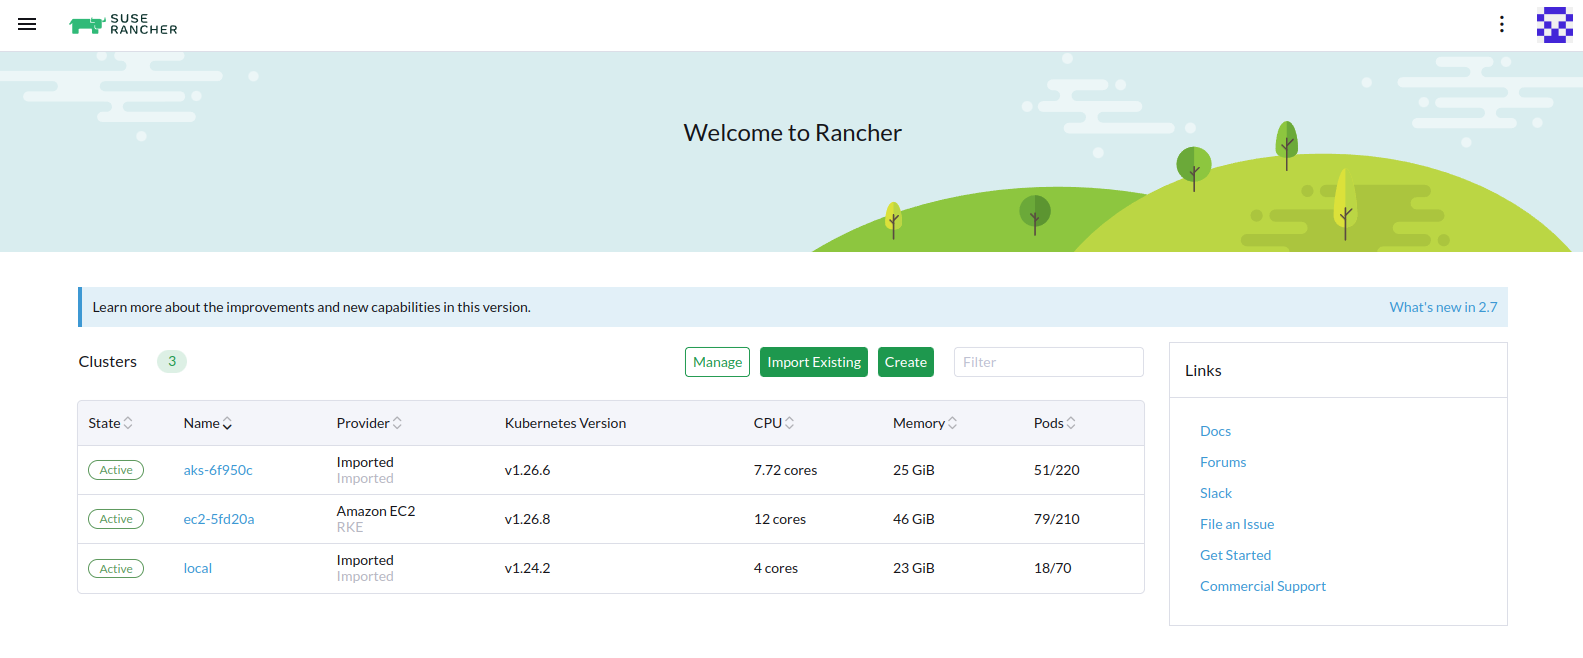
\includegraphics[width=\linewidth]{images/rancher-dashboard.png}
\label{fig:rancherDashboard}
\end{figure}

We will use Rancher's integrated CIS benchmarks for further analysis.

\subsubsection{Cluster Management Tools}

CIS Scans are one of the available cluster management applications within Rancher.

The Rancher CIS Benchmark uses \href{https://github.com/aquasecurity/kube-bench}{kube-bench}, an open-source tool from \href{https://www.aquasec.com/}{Aqua Security}, to check clusters for CIS Kubernetes Benchmark compliance. To generate a cluster-wide report, the application utilizes \href{https://sonobuoy.io/}{Sonobuoy} for report aggregation.\footnote{See \textit{Rancher Labs (2024)}: CIS Scans. \cite{rancherBenchmarks}}

Rancher includes many Benchmark profiles to support the various support versions of downstream Kubernetes clusters.

\subsubsection{CIS Scans Installation}

CIS Benchmarks can be installed within the Rancher UI as a Cluster Management application or using Infrastructure-as-Code automation, e.g., \href{https://www.terraform.io/}{Terraform}.

\begin{lstlisting}[caption=Installing CIS Benchmarks, frame=single, basicstyle=\ttfamily]
# CIS Benchmarks
resource "rancher2_app_v2" "cisbench_fom" {
  lifecycle {
    ignore_changes = all
  }
  cluster_id = rancher2_cluster.cluster_fom.id
  name = "rancher-cis-benchmark"
  namespace = "cis-operator-system"
  project_id = data.rancher2_project.system.id
  repo_name = "rancher-charts"
  chart_name = "rancher-cis-benchmark"
  chart_version = var.cischart
}
\end{lstlisting}

\subsubsection{CIS Scans Reports}

After installation, the CIS Benchmarks are available within the GUI for manual or scheduled executions.

\begin{figure}[H]
\centering
\caption {CIS Scans}
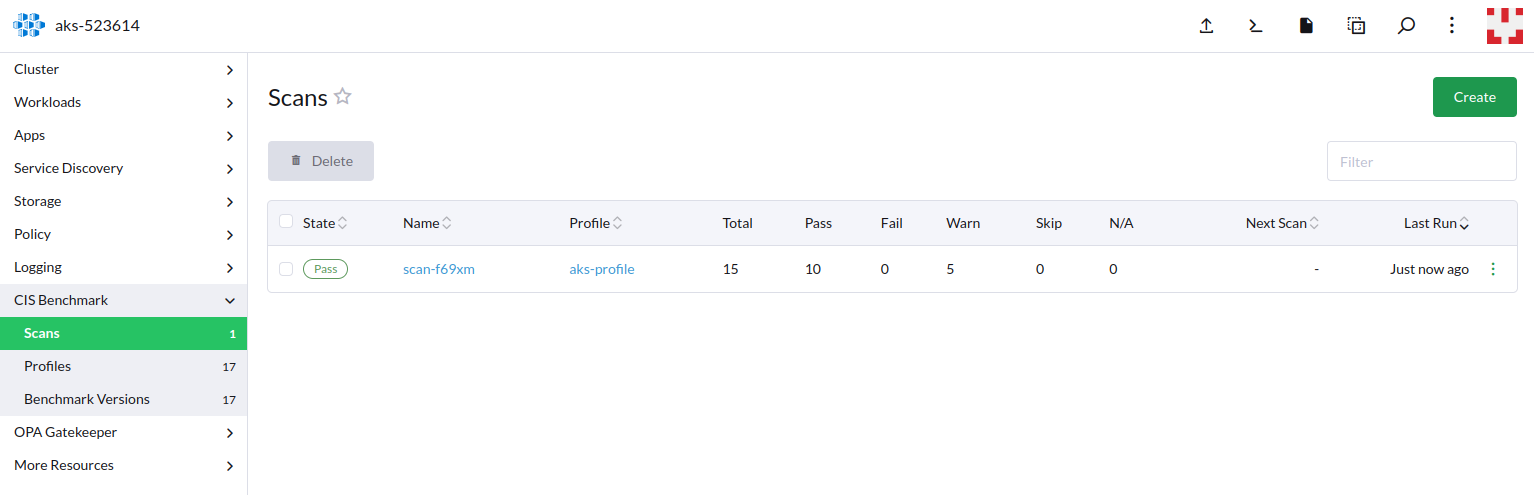
\includegraphics[width=\linewidth]{images/cis-scans-1.png}
\label{fig:cisScans}
\end{figure}

After a scan, the results will also be available in the GUI.

\begin{figure}[H]
\centering
\caption {CIS Scans Results AKS}
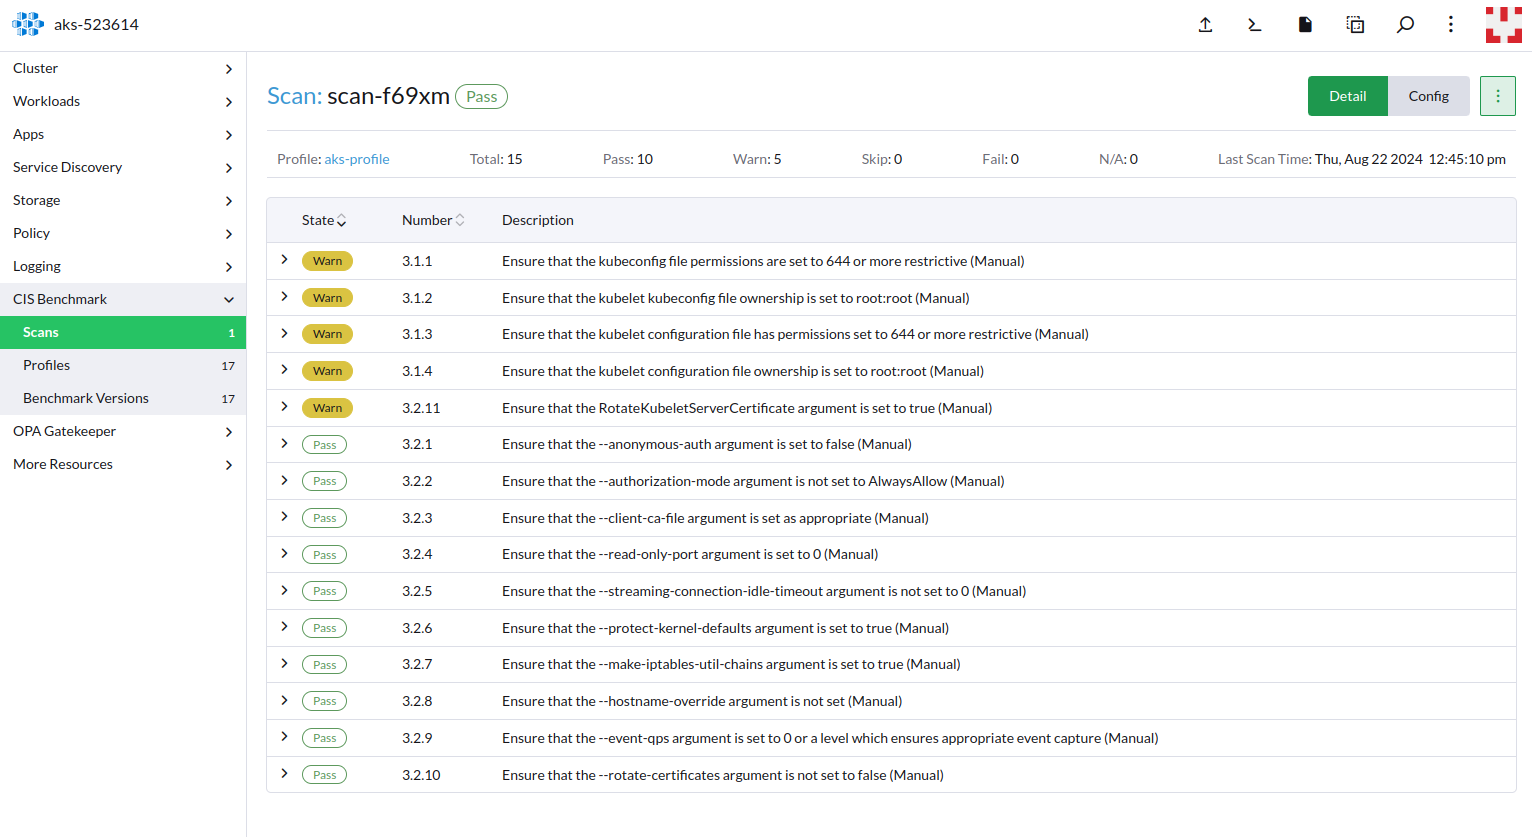
\includegraphics[width=\linewidth]{images/cis-scans-2.png}
\label{fig:cisAKS}
\end{figure}
